\documentclass{article}
\usepackage[utf8]{inputenc}

\title{Effective Approaches to Attention-based Neural Machine Translation}
\author{}
\date{}

\usepackage{natbib}
\usepackage{graphicx}
\usepackage{amsmath}
\usepackage[left=2.5cm,right=2.5cm,top=1cm,bottom=1.25cm]{geometry}
\usepackage{hyperref}
\usepackage{float}
\usepackage[export]{adjustbox}



\hypersetup{colorlinks=true,urlcolor=blue}
\pagenumbering{gobble}

\begin{document}

\maketitle

\section*{Link}
\href{https://arxiv.org/abs/1404.2188}{arXiv} 

\section*{Summary}
\begin{itemize}
    \item The paper studies two novel attention based models with simplicity and effectiveness in mind
    \begin{enumerate}
        \item Global attention where all source words are attended. A variable-length alignment vector $\textbf{a}_t$ whose size equals the number of time steps on source side is calculated by comparing current target hidden state $\textbf{h}_t$ and each source hidden state $\overline{\textbf{h}}_s$. Given the alignment vector the context vector $c_t$ is computed as the weighted average over all the source hidden states.
        \begin{figure}[H]
            \centering
            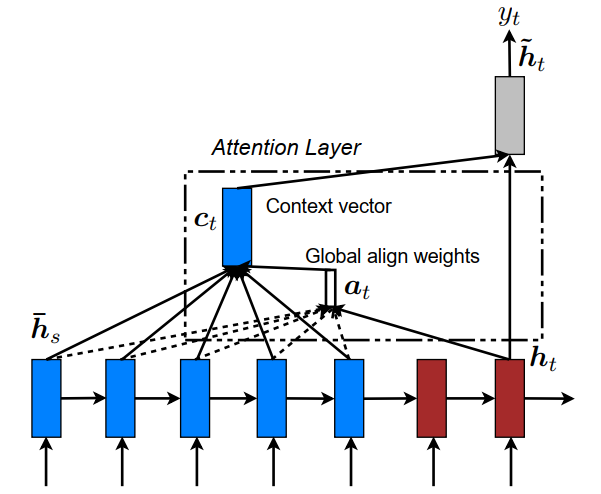
\includegraphics[scale=0.7]{global_attention.png}
            \caption{Global attention model}
            \label{fig:Figure 1}
        \end{figure}
        \item Global attention model which chooses to focus only on a small subset of source input positions per target words. This avoids the expensive computation incurred by global attention and is easier to train than hard attention which selects only one position per target and is non-differentiable. For local attention first an aligned position $p_t$ is generated for each target word at time $t$. The context vector is then derived as weighted average of the source hidden states withing window $[p_t-D, p_t+D]$.
        \begin{figure}[H]
            \centering
            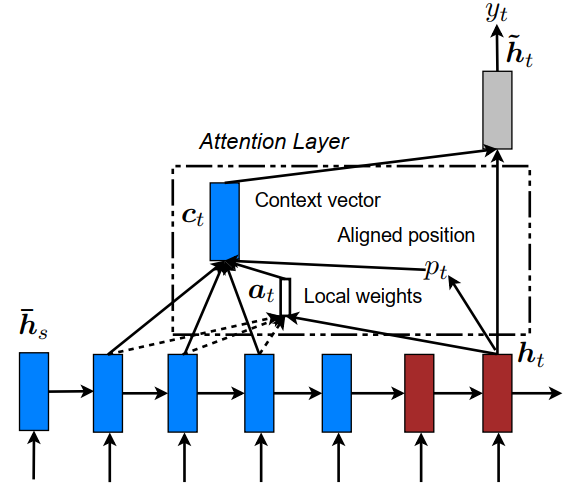
\includegraphics[scale=0.7]{local_attention.png}
            \caption{Local attention model}
            \label{fig:Figure 2}
        \end{figure}
        \end{enumerate}
    \item To make alignment decisions dependent on past decisions, they use an input-feeding approach in which attention vectors are concatenated with inputs at the next time steps.
    \begin{figure}[H]
        \centering
        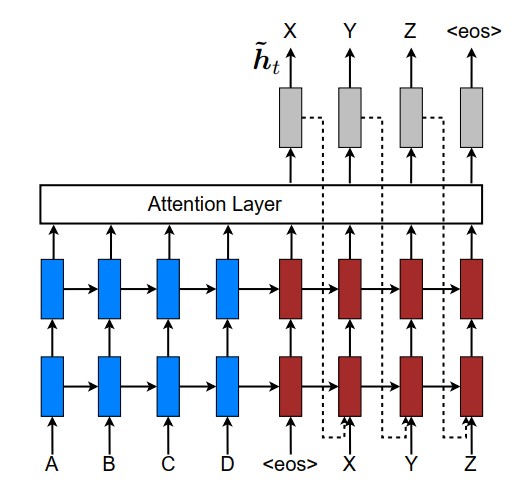
\includegraphics[scale=0.7]{input_feeding.png}
        \caption{Input-feeding approach}
        \label{fig:Figure 3}
    \end{figure}
    \item Local attention approach perform better than global attention approach which works significantly better than no attention approach. Source sentence reversing and input feeding approach also improves performance. Unknown replacement approach (replacing words not present in vocabulary with $<unk>$ further improves result. This shows that the attention models can learn useful alignment for unknown words.
    
\end{itemize}

\end{document}
